\begin{figure}[H]
\centering
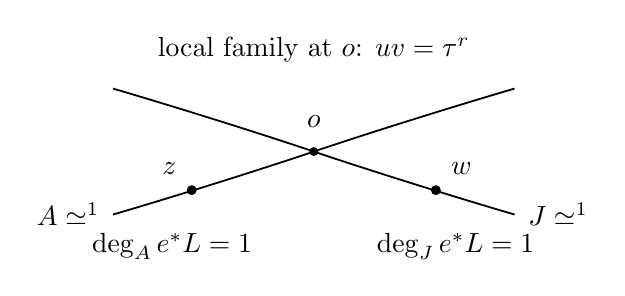
\begin{tikzpicture}[x=1cm,y=1cm,>=stealth]
  \draw[line width=0.65pt] (-2.55,-.80) .. controls (-1.7,-.55) and
    (-.65,-.22) .. (0,0) .. controls (.65,.22) and (1.7,.55) .. (2.55,.80);
  \draw[line width=0.65pt] (-2.55,.80) .. controls (-1.7,.55) and
    (-.65,.22) .. (0,0) .. controls (.65,-.22) and (1.7,-.55) .. (2.55,-.80);
  \node[anchor=east] at (-2.60,-.80) {$A\simeq\PP^1$};
  \node[anchor=west] at (2.60,-.80) {$J\simeq\PP^1$};
  \node at (-1.8,-1.20) {$\deg_A e^*L=1$};
  \node at (1.8,-1.20) {$\deg_J e^*L=1$};
  \fill (0,0) circle (1.6pt);
  \node[above=5pt] at (0,0) {$o$};
  \fill (-1.55,-.49) circle (1.8pt);
  \node[above left=2pt] at (-1.55,-.49) {$z$};
  \fill (1.55,-.49) circle (1.8pt);
  \node[above right=2pt] at (1.55,-.49) {$w$};
  \node at (0,1.30) {local family at $o$: $uv=\tau^r$};
\end{tikzpicture}
\caption{The split special source $A\cup J$, shown schematically.
The two crossing curves represent the rational components of contact
degree one. Their square has component types $A\times A$, $A\times J$,
$J\times A$ and $J\times J$.
The displayed pair $(z,w)$ lies in the mixed component $A\times J$
of the source square; this is one of the two component types where
the bivector may have a pole. The evaluation points are not stability
marks: either may also lie at the node, and they may coincide.
The picture represents the source curve, not its image in $X$.
The bounds in Equation~\eqref{ext:pole-table} and the contact vanishing
of Lemma~\ref{ext:contact-order} explain the cancellation.}
\label{fig:unmarked-boundary}
\end{figure}
